\chapter[Cenários de Teste]{Cenários de Teste}
\label{sec:cenarios_teste}
O principal objetivo dos cenários de teste é apoiar a observação e a análise sistemática da técnica de auto-localização utilizada durante o trabalho, assim como as diferentes configurações do ambiente e
do filtro utilizado.

Após a realização de todos os cenários de teste propostos, foi possível chegar a uma conclusão quanto à viabilidade da utilização da técnica do Filtro de Partículas em um contexto típico da Robótica Educacional.

Os cenários de teste consistem em cinco situações, nas quais a solução foi analisada, variando entre elas o ambiente e a configuração do filtro. Buscando
analisar a exatidão da auto-localização obtida em cada contexto, reiterando que o objetivo da pesquisa é analisar a viabilidade da utilização
de uma técnica de SLAM em um contexto típico da Robótica Educacional.

O Filtro de Partículas é uma das duas principais técnicas que buscam solucionar o problema
de SLAM. Por este motivo, os cenários de teste desta pesquisa buscam analisar o Filtro de Partículas, sendo esse executado no contexto da Robótica Educacional.
A intenção é viabilizar, em parte, a aplicação da solução de SLAM nesse contexto.

Os dados obtidos a partir de cada cenário de teste está organizado de acordo com a Tabela \ref{tab:org_dados}.

\begin{table}[H]
  \centering
  \caption{Organização dos Dados}
  \label{tab:org_dados}
  \begin{tabular}{|c|c|c|c|c|c|}
  \hline
  \textbf{Ex.} & \textbf{Partículas} & \textbf{Rotação} & \textbf{Deslocamento} & \textbf{Ciclos} & \textbf{Precisão} \\ \hline
  \end{tabular}
\end{table}

Onde,
\begin{itemize}
  \item \textbf{Ex.} faz referência ao ciclo de teste. Cada cenário foi testado 5 (cinco) vezes, buscando obter a média como resultado
  final do cenário;

  \item \textbf{Partículas} informa a quantidade de partículas utilizada durante este teste;

  \item \textbf{Rotação} informa a velocidade de rotação do robô, em graus por segundo;

  \item \textbf{Deslocamento} informa a velocidade de deslocamento em linha reta, em centímetros por segundo;

  \item \textbf{Ciclos} apresenta o número de ciclos de filtragem que foram necessários para obtenção da localização;

  \item \textbf{Posição} informando qual a posição estimada do robô, informando a margem de erro da posição estimada, tanto no eixo X
  quanto no eixo Y. Basicamente, este campo informa de que ponto a que ponto nos eixos X e Y, o robô pode estar localizado, utilizando o
  centímetro como unidade, seguindo o padrão do restante da pesquisa.

  \item \textbf{Precisão} informando qual a precisão obtida no teste, classificada em \textit{Ótima}, \textit{Boa}, \textit{Mediana},
  \textit{Baixa} e \textit{Baixíssima}. A classificação da precisão é feita a partir da comparação entre a posição estimada e a posição real.
  Como a posição estimada possui uma margem de erro, destacada como uma elipse no local indicado, a comparação utiliza como referência
  esta elipse, assim como a partícula definida como sendo a que possui os dados mais próximos aos obtidos pelo robô real. A classificação
  segue a tabela \ref{tab:class_precisao}.

  \begin{table}[H]
    \centering
    \caption{Classificação da Precisão.}
    \label{tab:class_precisao}
    \begin{tabular}{|c|c|}
    \hline
    \textbf{Precisão} & \textbf{Descrição}                                                                                                                                                                \\ \hline
    Ótima             & \begin{tabular}[c]{@{}c@{}}Posição real se encontra a menos \\ de 5 centímetros da partícula final.\end{tabular}                                                                  \\ \hline
    Boa               & \begin{tabular}[c]{@{}c@{}}Posição real se encontra a uma distância entre\\ 6 e 10 centímetros da partícula real, se encontrando,\\ ainda, dentro da elipse de erro.\end{tabular} \\ \hline
    Mediana           & \begin{tabular}[c]{@{}c@{}}Posição real se encontra próxima as fronteiras da\\ elipse de erro, com mais de 10 centímetros de distância\\ da partícula final.\end{tabular}         \\ \hline
    Baixa             & \begin{tabular}[c]{@{}c@{}}Posição real se encontra fora da elipse de erro, porém\\ a até 10 centímetros de distância da sua fronteira.\end{tabular}                              \\ \hline
    Baixíssima        & \begin{tabular}[c]{@{}c@{}}Posição real se encontra fora da elipse de erro, a uma\\ distância de mais de 10 centímetros da fronteira da elipse.\end{tabular}                      \\ \hline
    \end{tabular}
  \end{table}

\end{itemize}

Durante os cenários de teste, o ambiente utilizado foi o apresentado na Figura \ref{img:map1}, na qual todos os
valores se encontram em centímetros (cm).

\begin{figure}[H]
	\centering
	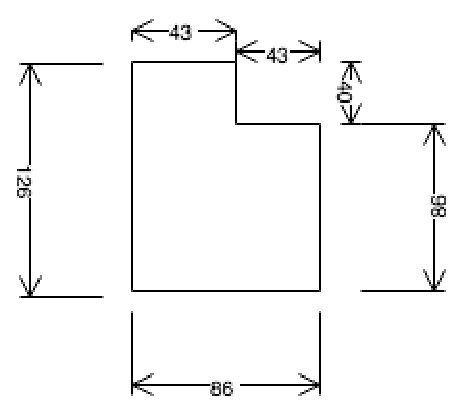
\includegraphics[scale=1.3]{figuras/map1.eps}
	\caption[Primeiro Cenário de Teste]{Mapa utilizado durante primeiro cenário de teste.}
	\label{img:map1}
\end{figure}

\subsection{Cenário de Teste 1}

Os resultados obtidos com o cenário estão dispostos na Tabela \ref{tab:cen1}. Deve-se atentar que o exemplo 3 possui um agravante, o
robô teve sua roda direita presa na parede, enquanto se locomovia. Desse modo, o robô perdeu-se e teve que se encontrar novamente, comportando-se
da maneira esperada em um caso básico de "sequestro do robô".

Este cenário faz referência à variação da quantidade de partículas.

\begin{table}[H]
\centering
\caption{Resultados Obtidos - Cenário 1}
\label{tab:cen1}
\begin{tabular}{|c|c|c|c|c|c|c|}
\hline
\textbf{Ex.} & \textbf{Partículas} & \textbf{Rotação} & \textbf{Deslocamento} & \textbf{Ciclos} & \textbf{Posição}                                            & \textbf{Precisão} \\ \hline
1                & 200                 & 100              & 100                   & 9                   & \begin{tabular}[c]{@{}c@{}}X: 25 a 70\\ Y: 15 a 30\end{tabular} & Ótima             \\ \hline
2                & 400                 & 100              & 100                   & 10                  & \begin{tabular}[c]{@{}c@{}}X: 17 a 37\\ Y: 39 a 66\end{tabular} & Boa               \\ \hline
3                & 500                 & 100              & 100                   & 21                  & \begin{tabular}[c]{@{}c@{}}X: 35 a 54\\ Y: 34 a 82\end{tabular} & Mediana           \\ \hline
4                & 100                 & 100              & 100                   & 5                   & \begin{tabular}[c]{@{}c@{}}X: 50 a 63\\ Y: 39 a 69\end{tabular} & Mediana           \\ \hline
5                & 150                 & 100              & 100                   & 3                   & \begin{tabular}[c]{@{}c@{}}X: 74 a 76\\ Y: 66 a 69\end{tabular} & Ótima             \\ \hline
\end{tabular}
\end{table}


\subsection{Cenário de Teste 2}

Os resultados obtidos com o cenário estão dispostos na Tabela \ref{tab:cen2}. Este cenário faz referência à variação da velocidade de
rotação do robô.

\begin{table}[H]
\centering
\caption{Resultados Obtidos - Cenário 2}
\label{tab:cen2}
\begin{tabular}{|c|c|c|c|c|c|c|}
\hline
\textbf{Ex.} & \textbf{Partículas} & \textbf{Rotação} & \textbf{Deslocamento} & \textbf{Ciclos} & \textbf{Posição}                                            & \textbf{Precisão} \\ \hline
1                & 150                 & 10               & 100                   & 7                   & \begin{tabular}[c]{@{}c@{}}X: 30 a 72\\ Y: 47 a 71\end{tabular} & Boa               \\ \hline
2                & 150                 & 30               & 100                   & 6                   & \begin{tabular}[c]{@{}c@{}}X: 20 a 38\\ Y: 42 a 67\end{tabular} & Ótima             \\ \hline
3                & 150                 & 50               & 100                   & 3                   & \begin{tabular}[c]{@{}c@{}}X: 29 a 63\\ Y: 30 a 62\end{tabular} & Boa               \\ \hline
4                & 150                 & 70               & 100                   & 3                   & \begin{tabular}[c]{@{}c@{}}X: 23 a 66\\ Y: 29 a 68\end{tabular} & Mediana           \\ \hline
5                & 150                 & 90               & 100                   & 8                   & \begin{tabular}[c]{@{}c@{}}X: 36 a 61\\ Y: 15 a 35\end{tabular} & Mediana           \\ \hline
\end{tabular}
\end{table}


\subsection{Cenário de Teste 3}

Os resultados obtidos com o cenário estão dispostos na Tabela \ref{tab:cen3}. Este cenário faz referência à variação da velocidade de
deslocamento do robô, em unidades do diâmetro das rodas por segundo. Fixou-se a quantidade de partículas em 150, de acordo com os resultados
obtidos nos cenários anteriores, assim como a velocidade de rotação em 30 graus por segundo.

\begin{table}[H]
\centering
\caption{Resultados Obtidos - Cenário 3}
\label{tab:cen3}
\begin{tabular}{|c|c|c|c|c|c|c|}
\hline
\textbf{Ex.} & \textbf{Partículas} & \textbf{Rotação} & \textbf{Deslocamento} & \textbf{Ciclos} & \textbf{Posição}                                            & \textbf{Precisão} \\ \hline
1                & 150                 & 30               & 2                     & 4                   & \begin{tabular}[c]{@{}c@{}}X: 30 a 70\\ Y: 28 a 62\end{tabular} & Baixa             \\ \hline
2                & 150                 & 30               & 5                     & 6                   & \begin{tabular}[c]{@{}c@{}}X: 31 a 59\\ Y: 32 a 70\end{tabular} & Mediana           \\ \hline
3                & 150                 & 30               & 10                    & 3                   & \begin{tabular}[c]{@{}c@{}}X: 30 a 73\\ Y: 20 a 78\end{tabular} & Baixa             \\ \hline
4                & 150                 & 30               & 15                    & 6                   & \begin{tabular}[c]{@{}c@{}}X: 82 a 89\\ Y: 73 a 82\end{tabular} & Boa               \\ \hline
5                & 150                 & 30               & 30                    & 5                   & \begin{tabular}[c]{@{}c@{}}X: 23 a 54\\ Y: 40 a 73\end{tabular} & Mediana           \\ \hline
\end{tabular}
\end{table}

\subsection{Cenário de Teste 4}

Os resultados obtidos com o cenário estão dispostos na Tabela \ref{tab:cen4}. Este cenário faz referência à análise da solução
utilizando a configuração que obteve os melhores resultados nos cenários anteriores, ou seja:

\begin{itemize}
  \item \textbf{Partículas:} 150
  \item \textbf{Rotação:} 30
  \item \textbf{Deslocamento:} 15
\end{itemize}

O objetivo principal deste cenário é verificar a variabilidade dos resultados utilizando configuração fixa durante os exemplos.

\begin{table}[H]
\centering
\caption{Resultados Obtidos - Cenário 4}
\label{tab:cen4}
\begin{tabular}{|c|c|c|c|c|c|c|}
\hline
\textbf{Ex.} & \textbf{Partículas} & \textbf{Rotação} & \textbf{Deslocamento} & \textbf{Ciclos} & \textbf{Posição}                                            & \textbf{Precisão} \\ \hline
1                & 150                 & 30               & 15                    & 8                   & \begin{tabular}[c]{@{}c@{}}X: 30 a 54\\ Y: 28 a 45\end{tabular} & Mediana           \\ \hline
2                & 150                 & 30               & 15                    & 4                   & \begin{tabular}[c]{@{}c@{}}X: 62 a 87\\ Y: 23 a 58\end{tabular} & Baixa             \\ \hline
3                & 150                 & 30               & 15                    & 5                   & \begin{tabular}[c]{@{}c@{}}X: 27 a 75\\ Y: 10 a 32\end{tabular} & Baixíssima        \\ \hline
4                & 150                 & 30               & 15                    & 7                   & \begin{tabular}[c]{@{}c@{}}X: 66 a 70\\ Y: 27 a 33\end{tabular} & Mediana           \\ \hline
5                & 150                 & 30               & 15                    & 8                   & \begin{tabular}[c]{@{}c@{}}X: 37 a 67\\ Y: 34 a 67\end{tabular} & Boa               \\ \hline
\end{tabular}
\end{table}

\subsection{Cenário de Teste 5}

Os resultados obtidos com o cenário estão dispostos na Tabela \ref{tab:cen5}. Este cenário faz referência a análise da solução
utilizando um mapa sem características únicas, como um retângulo.

\begin{itemize}
  \item \textbf{Partículas:} 150
  \item \textbf{Rotação:} 30
  \item \textbf{Deslocamento:} 15
\end{itemize}

O objetivo deste cenário é verificar a viabilidade da utilização do Filtro de Partículas em um ambiente sem pontos de referência únicos.

\begin{table}[H]
\centering
\caption{Resultados Obtidos - Cenário 5}
\label{tab:cen5}
\begin{tabular}{|c|c|c|c|c|c|c|}
\hline
\textbf{Ex.} & \textbf{Partículas} & \textbf{Rotação} & \textbf{Deslocamento} & \textbf{Ciclos} & \textbf{Posição}                                            & \textbf{Precisão} \\ \hline
1                & 150                 & 30               & 15                    & 6                   & \begin{tabular}[c]{@{}c@{}}X: 21 a 63\\ Y: 40 a 84\end{tabular} & Mediana           \\ \hline
2                & 150                 & 30               & 15                    & 11                   & \begin{tabular}[c]{@{}c@{}}X: 37 a 70\\ Y: 47 a 90\end{tabular} & Mediana             \\ \hline
3                & 150                 & 30               & 15                    & 6                   & \begin{tabular}[c]{@{}c@{}}X: 27 a 75\\ Y: 10 a 32\end{tabular} & Mediana        \\ \hline
4                & 150                 & 30               & 15                    & 7                   & \begin{tabular}[c]{@{}c@{}}X: 66 a 70\\ Y: 27 a 33\end{tabular} & Mediana           \\ \hline
5                & 150                 & 30               & 15                    & 11                   & \begin{tabular}[c]{@{}c@{}}X: 37 a 67\\ Y: 34 a 67\end{tabular} & Mediana               \\ \hline
\end{tabular}
\end{table}
